\documentclass[12pt, letterpaper]{article}
\usepackage[margin=1in]{geometry}
\usepackage[T1]{fontenc}
\usepackage{lmodern}
\usepackage{cmap}
\usepackage[utf8]{inputenc}
\usepackage{amsmath, amssymb, amsthm}
\usepackage{mathtools}
\usepackage{enumitem}
\usepackage{booktabs}
\usepackage{xcolor}
\usepackage{titlesec}
\usepackage{parskip}
\usepackage{hyperref}
\usepackage{fancyhdr}
\usepackage{tcolorbox}
\usepackage{graphicx}
\usepackage{caption}
\tcbuselibrary{skins, breakable}

\definecolor{darkblue}{RGB}{15,55,115}
\definecolor{midblue}{RGB}{30,100,180}
\definecolor{theorybg}{RGB}{245,250,255}
\definecolor{questionbg}{RGB}{255,252,240}
\definecolor{evencolor}{RGB}{60,0,100}

\hypersetup{colorlinks=true,linkcolor=darkblue,urlcolor=midblue,
  pdftitle={Kurlat --- A Course in Modern Macroeconomics --- Complete Solutions, Chapter 6}}

\setlength{\headheight}{14pt}
\pagestyle{fancy}
\fancyhf{}
\renewcommand{\headrulewidth}{0.4pt}
\fancyhead[L]{\small\textcolor{darkblue}{\textit{Kurlat --- A Course in Modern Macroeconomics}}}
\fancyhead[R]{\small\textcolor{darkblue}{\thepage}}
\fancyfoot[C]{\small\textcolor{gray}{Complete Solutions --- Chapter 6}}

\titleformat{\section}[block]
  {\large\bfseries\color{darkblue}}{}{0pt}{}
  [\vspace{2pt}\color{darkblue}\rule{\textwidth}{1.5pt}\vspace{4pt}]

\titleformat{\subsection}[block]
  {\normalsize\bfseries\color{midblue}}{}{0pt}{}
  [\vspace{1pt}\color{midblue}\rule{0.5\textwidth}{0.8pt}\vspace{3pt}]

\tcbset{
  theorybox/.style={
    enhanced,breakable,colback=theorybg,colframe=darkblue,
    fonttitle=\bfseries\small\color{darkblue},boxrule=0.5pt,arc=3pt,
    left=6pt,right=6pt,top=4pt,bottom=4pt,title={Key Theory},
  },
  questionbox/.style={
    enhanced,breakable,colback=questionbg,colframe=gray!60,
    fonttitle=\bfseries\small\color{gray!60!black},boxrule=0.4pt,arc=2pt,
    left=6pt,right=6pt,top=4pt,bottom=4pt,title={\textit{Question}},
  },
  oddbox/.style={
    enhanced,breakable,colback=white,colframe=darkblue,
    attach boxed title to top left={yshift=-2mm,xshift=6mm},
    boxed title style={colback=darkblue,colframe=darkblue,arc=2pt,
      boxrule=0pt,left=6pt,right=6pt,top=3pt,bottom=3pt},
    fonttitle=\bfseries\large\color{white},
    boxrule=0.8pt,arc=3pt,
    left=8pt,right=8pt,top=10pt,bottom=6pt,
  },
  evenbox/.style={
    enhanced,breakable,colback=white,colframe=evencolor,
    attach boxed title to top left={yshift=-2mm,xshift=6mm},
    boxed title style={colback=evencolor,colframe=evencolor,arc=2pt,
      boxrule=0pt,left=6pt,right=6pt,top=3pt,bottom=3pt},
    fonttitle=\bfseries\large\color{white},
    boxrule=0.8pt,arc=3pt,
    left=8pt,right=8pt,top=10pt,bottom=6pt,
  },
  databox/.style={
    enhanced,breakable,colback=gray!8,colframe=gray!55,
    fonttitle=\bfseries\small\color{gray!60!black},boxrule=0.4pt,arc=2pt,
    left=6pt,right=6pt,top=4pt,bottom=4pt,title={Numerical exercise --- see the companion code},
  },
  trapbox/.style={
    enhanced,breakable,colback=red!4,colframe=red!45!black,
    fonttitle=\bfseries\small\color{white},boxrule=0.4pt,arc=2pt,
    coltitle=white,
    left=6pt,right=6pt,top=4pt,bottom=4pt,title={Where this goes wrong},
  },
}

\newcommand{\pd}[2]{\dfrac{\partial #1}{\partial #2}}
\newcommand{\dd}[2]{\dfrac{d #1}{d #2}}
\newcommand{\MRS}{\mathrm{MRS}}
\newcommand{\MRT}{\mathrm{MRT}}
\newcommand{\MU}{\mathrm{MU}}
\newcommand{\Var}{\mathrm{Var}}
\newcommand{\Cov}{\mathrm{Cov}}
\newcommand{\E}{\mathrm{E}}
\newcommand{\MPK}{\mathrm{MPK}}
\newcommand{\MPL}{\mathrm{MPL}}
\newcommand{\stst}{^{\ast}}
\newcommand{\EST}{^{\mathrm{EST}}}
\newcommand{\TRUE}{^{\mathrm{TRUE}}}

\setlist[enumerate,1]{label=(\alph*),itemsep=6pt,parsep=2pt}
\setlist[enumerate,2]{label=(\roman*),itemsep=3pt}

\begin{document}

%======================================================================
% TITLE PAGE
%======================================================================
\begin{titlepage}
\centering
\vspace*{2.5cm}
{\Huge\bfseries\color{darkblue} A Course in Modern Macroeconomics\par}
\vspace{6pt}
{\large Pablo Kurlat (2020)\par}
\vspace{1.4cm}
{\LARGE\bfseries Complete Solutions\par}
\vspace{6pt}
{\LARGE\bfseries Chapter 6 --- Consumption and Saving\par}
\vspace{1.2cm}
{\large All nine end-of-chapter problems, 6.1--6.9 (pp.~121--125)\par}
\vspace{2cm}

\begin{tcolorbox}[theorybox,title={What is in this file},width=0.86\textwidth]
\small
Every problem carries the full question text, a step-by-step solution with no skipped
algebra, an economic reading of the result, and a verification. Numerical answers are
reproduced by the companion scripts in \texttt{Resolucao/kurlat\_ch06\_codigo/}, which
check each analytical formula against an independent computation --- in most cases a direct
numerical maximisation of the household's problem --- and abort on any mismatch.

\smallskip
Problems are grouped by \textbf{topic}, not by number, following the order of the
chapter's own sections. Blue boxes are odd-numbered problems, purple boxes even.

\smallskip
\textbf{Kurlat publishes no answer key}, so every result here is verified by other means:
executed numerical checks (marked \checkmark), the Euler equation and budget constraint
substituted back, limiting cases ($\sigma\to1$, $m\to0$, $\beta(1+r)\to1$), and cross-book
comparison with Romer (2012) ch.~8 and Jones (2020) ch.~16, both in \texttt{Livros/}.

\smallskip
Companion to \texttt{kurlat\_solutions\_ch1-4.tex}, \texttt{...\_ch05.tex} and
\texttt{...\_ch09.tex}. Chapter 8 is outside the course syllabus.
\end{tcolorbox}

\vfill
{\small MPE Insper --- Macroeconomia I --- 2026, 3\textordmasculine{} trimestre \quad$\cdot$\quad
Aula 4 --- Lista 3\par}
\end{titlepage}

\tableofcontents
\newpage

%======================================================================
\section{Chapter 6 \quad Consumption and Saving}
%======================================================================

\begin{tcolorbox}[theorybox,title={Chapter 6 Overview}]
The Solow model assumed a saving rate. This chapter derives one. Everything in it follows
from a single optimisation problem and its two implications.

\smallskip
\textbf{The problem.} A household chooses $c_1$, $c_2$ (and savings $a$) to maximise
$u(c_1)+\beta u(c_2)$ subject to $a=y_1-c_1$ and $c_2=y_2+(1+r)a$. Collapsing the two
constraints gives the \emph{intertemporal budget constraint}
\[
c_1+\frac{c_2}{1+r}=y_1+\frac{y_2}{1+r} .
\tag{6.2.4}
\]

\smallskip
\textbf{Implication 1: the Euler equation.} The first-order conditions give
\[
u'(c_1)=\beta(1+r)\,u'(c_2) ,
\tag{6.2.8}
\]
the single most-used equation in modern macroeconomics. It says the marginal cost of giving
up a unit today equals the discounted marginal benefit of the $(1+r)$ units it buys
tomorrow, and it reappears verbatim as (6.3.9), (7.4.3) and (9.1.8).

\smallskip
\textbf{Implication 2: the permanent income hypothesis.} With CRRA utility
$u(c)=c^{1-\sigma}/(1-\sigma)$ the Euler equation gives $c_2=[\beta(1+r)]^{1/\sigma}c_1$
and, substituted into (6.2.4),
\[
c_1=\frac{y_1+\dfrac{1}{1+r}y_2}
         {\underbrace{1+\dfrac{1}{1+r}\left[\beta(1+r)\right]^{\frac{1}{\sigma}}}_{\textstyle\Omega}}
\tag{6.2.9}
\]
Consumption is proportional to the \emph{present value of lifetime income}, not to current
income. Everything the chapter says about the marginal propensity to consume, about the
Keynesian consumption function, and about fiscal policy is read off this one formula.

\smallskip
\textbf{The notation used throughout this file.} It is convenient to name the denominator
of (6.2.9) once:
\[
\Omega\equiv 1+\beta^{\frac{1}{\sigma}}(1+r)^{\frac{1-\sigma}{\sigma}}
=1+\frac{1}{1+r}\left[\beta(1+r)\right]^{\frac{1}{\sigma}} ,
\qquad
W\equiv a_0+y_1-\tau_1+\frac{y_2-\tau_2}{1+r},
\]
so that $c_1=W/\Omega$. Note that $\Omega>1$ always, that $\Omega$ is increasing in $\beta$,
and that $\Omega$ is increasing, constant or decreasing in $r$ according as
$\sigma\lessgtr1$. That last fact drives Problems 6.1(e), 6.3 and 6.6.

\smallskip
\textbf{Two parameters, and do not confuse them.} $\beta$ is \emph{impatience}: it says how
much the household cares about the future at all. $\sigma$ is the inverse of the
\emph{elasticity of intertemporal substitution}, $\mathrm{EIS}=1/\sigma$: it says how
willing the household is to let consumption differ across dates in response to a price. A
patient household ($\beta$ high) saves more; a household with a low EIS ($\sigma$ high)
resists tilting its consumption path whatever the interest rate does.

\smallskip
\textbf{Where the model fails, and the two repairs.} The measured marginal propensity to
consume out of temporary income is far above what (6.2.9) predicts (Problem 6.8 makes the
gap explicit). \S6.2 adds \emph{credit constraints} (Problem 6.5) and \S6.4 sketches
\emph{behavioural} departures. Naming which repair is at work is how the chapter says
consumption policy should be analysed.
\end{tcolorbox}

%---- Topic: The Two-Period Problem and Its Comparative Statics ----
\subsection{The Two-Period Problem and Its Comparative Statics}

%------- 6.1 -------
% Topic: The Two-Period Problem and Its Comparative Statics
% Keywords: Euler equation, CRRA, closed form, intertemporal budget constraint, EIS
\begin{tcolorbox}[oddbox,title={Problem 6.1 \quad Two-Period Problem with Taxes and Initial Wealth}]
\begin{tcolorbox}[questionbox]
Suppose a household solves the following two-period consumption-savings problem with taxes:
\[
\max_{c_1,\,a,\,c_2}\ u(c_1)+\beta u(c_2)
\quad\text{s.t.}\quad
a=a_0+y_1-\tau_1-c_1,
\qquad
c_2=y_2-\tau_2+(1+r)a
\]
with $u(c)=\dfrac{c^{1-\sigma}}{1-\sigma}$, where $c_1$ is consumption at time 1, $c_2$ is
consumption at time 2, $y_1$ is household income at time 1, $y_2$ is household income at
time 2, $\tau_1$ are taxes at time 1, $\tau_2$ are taxes at time 2, and $a_0$ is initial
wealth.\\[3pt]
(a) Solve for the household's choice of $c_1$, $c_2$ and $a$ in closed form.\\[3pt]
(b) How does $c_1/y_1$ depend on $y_2$? What would happen if households suddenly became
optimistic about the future?\\[3pt]
(c) How does $c_1/y_1$ depend on $a_0$? Interpret.\\[3pt]
(d) How does $c_1/y_1$ depend on $\beta$? Interpret.\\[3pt]
(e) Suppose $y_2=\tau_1=\tau_2=0$ and compute $\partial c_1/\partial r$. How does the answer
depend on $\sigma$? Interpret the answer. [Hint: this is a hard question, not the maths but
the interpretation. Think about what $\sigma$ means for the relative importance of income
and substitution effects.]
\end{tcolorbox}

\textbf{Solution:}
\begin{enumerate}

\item \textbf{Step 1: collapse the two constraints.} Solve the second constraint for
$a=(c_2-y_2+\tau_2)/(1+r)$ and substitute into the first:
\[
c_1+\frac{c_2-y_2+\tau_2}{1+r}=a_0+y_1-\tau_1
\;\Longrightarrow\;
c_1+\frac{c_2}{1+r}=\underbrace{a_0+y_1-\tau_1+\frac{y_2-\tau_2}{1+r}}_{\textstyle W} .
\tag{6.1.1}
\]
This is (6.2.4) with taxes and initial wealth. Note where each term sits: $a_0$ enters
undiscounted because it is already available at date 1, while $y_2-\tau_2$ is discounted.

\smallskip
\textbf{Step 2: the Euler equation.} The Lagrangian for
$\max u(c_1)+\beta u(c_2)$ subject to (6.1.1) is
$\mathcal{L}=u(c_1)+\beta u(c_2)+\lambda\left[W-c_1-\frac{c_2}{1+r}\right]$, with
first-order conditions
\[
u'(c_1)=\lambda,
\qquad
\beta u'(c_2)=\frac{\lambda}{1+r}
\qquad\Longrightarrow\qquad
u'(c_1)=\beta(1+r)u'(c_2) .
\]
With $u'(c)=c^{-\sigma}$,
\[
c_1^{-\sigma}=\beta(1+r)c_2^{-\sigma}
\qquad\Longrightarrow\qquad
c_2=\left[\beta(1+r)\right]^{\frac{1}{\sigma}}c_1 .
\tag{6.1.2}
\]

\smallskip
\textbf{Step 3: substitute back.} Putting (6.1.2) into (6.1.1),
\[
c_1\left[1+\frac{\left[\beta(1+r)\right]^{1/\sigma}}{1+r}\right]=W
\qquad\Longrightarrow\qquad
c_1=\frac{W}{\Omega},
\qquad
\Omega\equiv1+\beta^{\frac{1}{\sigma}}(1+r)^{\frac{1-\sigma}{\sigma}} .
\]
Therefore
\[
\boxed{\;c_1=\frac{a_0+y_1-\tau_1+\dfrac{y_2-\tau_2}{1+r}}{\Omega}\;}
\qquad
\boxed{\;c_2=\left[\beta(1+r)\right]^{\frac{1}{\sigma}}\frac{W}{\Omega}\;}
\]
\[
\boxed{\;a=a_0+y_1-\tau_1-\frac{W}{\Omega}\;}
\]
\checkmark\ In \texttt{ch06\_numerico.py} this closed form is compared, for
$\sigma\in\{0.5,1,2,4\}$, against a direct numerical maximisation of
$u(c_1)+\beta u(c_2)$ over the budget line; the two agree to $10^{-6}$, and the Euler
equation and the budget constraint are each substituted back and verified.

\smallskip
\emph{Read the formula before doing any comparative statics.} It has exactly two moving
parts. The numerator $W$ is \textbf{lifetime resources}: it is where $y_1$, $y_2$, $a_0$ and
the two taxes live, and \emph{only their present value matters} --- the timing of income and
of taxes is irrelevant to it. The denominator $\Omega$ is \textbf{the shape of the plan}: it
is where $\beta$, $\sigma$ and $r$ live, and it determines how the given resources are split
between the two dates. Every part below is a question about one or the other.

\item \textbf{Dependence on $y_2$.} From the boxed formula,
\[
\frac{c_1}{y_1}=\frac{W}{\Omega y_1}
\qquad\Longrightarrow\qquad
\boxed{\pd{}{y_2}\left(\frac{c_1}{y_1}\right)=\frac{1}{\Omega(1+r)y_1}>0} .
\]
\checkmark\ Confirmed by finite differences for every $\sigma$ tested.

\smallskip
\emph{If households suddenly became optimistic about the future}, $y_2$ rises in
expectation, so $c_1$ rises \textbf{today}, with no change whatsoever in today's income. The
saving rate $s=1-c_1/y_1$ falls. This is the sharpest break with the Keynesian consumption
function: consumption can boom on news alone. It is the reason consumer-confidence indices
are watched, and the reason a credible announcement of future tax cuts, or of a future
productivity boom, moves spending immediately --- exactly the mechanism that Problem 9.9 and
the anticipated-technology experiment of \S9.3 run in general equilibrium.

\item \textbf{Dependence on $a_0$.}
\[
\boxed{\pd{}{a_0}\left(\frac{c_1}{y_1}\right)=\frac{1}{\Omega y_1}>0}
\]
\checkmark\ Note this derivative is larger than the one in part (b) by a factor $(1+r)$,
because initial wealth is available now and future income has to be discounted.

\smallskip
\emph{Interpretation.} The ratio of consumption to current income is \textbf{not a
preference parameter}. Two households with identical $\beta$, $\sigma$ and current income
will have different saving rates if their balance sheets differ. Three consequences:
\begin{itemize}[leftmargin=1.3em,itemsep=2pt,topsep=3pt]
\item Cross-sectional saving rates cannot be read as evidence about thrift. The elderly have
      accumulated $a_0$ and so consume a high fraction of current income; the young have not.
\item There is a \textbf{wealth effect} on consumption: a rise in house or equity prices
      raises $a_0$ and therefore raises consumption immediately, without any change in
      income. This is one of the main channels through which asset markets reach the real
      economy.
\item Aggregate saving rates fall when aggregate wealth rises, which is one candidate
      explanation for the long decline of measured US household saving.
\end{itemize}

\item \textbf{Dependence on $\beta$.} $\beta$ appears only in $\Omega$:
\[
\pd{\Omega}{\beta}=\frac{1}{\sigma}\beta^{\frac{1}{\sigma}-1}(1+r)^{\frac{1-\sigma}{\sigma}}>0
\qquad\Longrightarrow\qquad
\boxed{\pd{}{\beta}\left(\frac{c_1}{y_1}\right)
=-\frac{W}{\Omega^{2}y_1}\pd{\Omega}{\beta}<0}
\]
\checkmark

\smallskip
\emph{Interpretation.} More patience means less consumption today and more saving, for
\emph{any} $\sigma$ and any $r$. This is the one comparative static in the whole problem
with an unambiguous sign, and the reason is structural: $\beta$ does not appear in $W$ at
all, so there is no offsetting wealth effect --- patience is a pure preference over the
shape of the path.

\item \textbf{Dependence on $r$, with $y_2=\tau_1=\tau_2=0$.} Now $W=a_0+y_1$ does not
depend on $r$, so all the action is in $\Omega$:
\[
\dd{\Omega}{r}=\beta^{\frac{1}{\sigma}}\,\frac{1-\sigma}{\sigma}\,
(1+r)^{\frac{1-2\sigma}{\sigma}} ,
\]
\[
\boxed{\;\dd{c_1}{r}=-\frac{a_0+y_1}{\Omega^{2}}\,\dd{\Omega}{r}
=-(a_0+y_1)\,\beta^{\frac{1}{\sigma}}\,\frac{1-\sigma}{\sigma}\,
\frac{(1+r)^{\frac{1-2\sigma}{\sigma}}}{\Omega^{2}}\;}
\]
Every factor is positive except $(1-\sigma)$, so
\[
\operatorname{sign}\dd{c_1}{r}=\operatorname{sign}(\sigma-1),
\]
that is,
\[
\sigma<1\Rightarrow c_1\ \text{falls},
\quad
\sigma=1\Rightarrow c_1\ \text{unchanged},
\quad
\sigma>1\Rightarrow c_1\ \text{rises}.
\]
\checkmark\ Verified by finite differences: with $y_1=1$, $a_0=0.2$, $\beta=0.96$,
$r=0.05$, $\dd{c_1}{r}$ equals $-0.2856$, $0$, $+0.1428$ and $+0.2142$ for
$\sigma=0.5,\,1,\,2,\,4$.

\smallskip
\emph{Interpretation --- and the hint is right that this is the hard part.} The household
here has all its income today and none tomorrow, so it must be a saver. A rise in $r$ is a
\textbf{fall in the price of future consumption}, $p_2=1/(1+r)$. Standard consumer theory
splits the response into two:

\begin{itemize}[leftmargin=1.3em,itemsep=4pt,topsep=4pt]
\item \textbf{Substitution effect.} Future consumption is cheaper, so tilt the plan towards
      it: $c_1$ down. Its strength is the elasticity of substitution between $c_1$ and
      $c_2$, which for CRRA is exactly $\mathrm{EIS}=1/\sigma$.
\item \textbf{Income effect.} At the old plan the household is better off --- its savings
      now buy more --- so it wants more of both goods: $c_1$ up.
\end{itemize}

The two are exactly balanced when the elasticity of substitution is one, which is
$\sigma=1$, the logarithmic case; then $\Omega=1+\beta$ and
$c_1=(a_0+y_1)/(1+\beta)$, with $r$ nowhere in sight. Away from that knife edge:
\begin{itemize}[leftmargin=1.3em,itemsep=2pt,topsep=3pt]
\item $\sigma<1$ (\textbf{high EIS}, the household is happy to let consumption differ across
      dates): substitution wins and saving rises with $r$. This is the intuitive case and
      the one most people expect.
\item $\sigma>1$ (\textbf{low EIS}, the household badly wants a smooth path): income wins and
      saving \emph{falls} when $r$ rises. The intuition is the ``target saver'': someone
      determined to reach a given standard of living tomorrow needs to set aside less today
      when the return is higher, and spends the difference.
\end{itemize}

\smallskip
This is why the sign of the aggregate saving response to interest rates is a genuinely open
empirical question rather than a theoretical one, and why estimates of the EIS occupy a
whole literature. Most microeconometric estimates put $1/\sigma$ below one, i.e.\ $\sigma>1$
--- the counterintuitive case. It is also why the sign of $\Omega$'s response to $r$ is
flagged in the chapter overview: it drives Problems 6.3 and 6.6 as well.

\end{enumerate}

\begin{center}
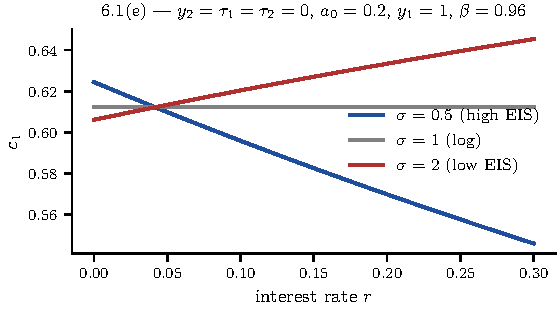
\includegraphics[width=0.72\linewidth]{fig/fig_k6_1_juros.pdf}\\[3pt]
\captionof{figure}{Problem 6.1(e). With all income in period 1, the response of $c_1$ to
the interest rate has the sign of $\sigma-1$. The logarithmic case is exactly flat.}
\label{fig:juros61}
\end{center}
\end{tcolorbox}

%------- 6.9 -------
% Topic: The Two-Period Problem and Its Comparative Statics
% Keywords: homotheticity, elasticity, permanent income, wealth share, proportional MPC
\begin{tcolorbox}[oddbox,title={Problem 6.9 \quad The Marginal Propensity to Consume in Proportional Terms}]
\begin{tcolorbox}[questionbox]
A household solves a special case of the problem in Exercise 6.1, with
$\tau_1=\tau_2=a_0=0$ and $y_2=my_1$, where $m$ is some number.\\[3pt]
(a) Suppose that both $y_1$ and $y_2$ increase by $x\%$. By what percentage do $c_1$ and
$c_2$ increase?\\[3pt]
(b) Suppose $y_1$ increases by $x\%$ but $y_2$ remains unchanged. By what percentage does
$c_1$ increase? How does this depend on $m$ and $r$? Explain.
\end{tcolorbox}

\textbf{Setup.} From Problem 6.1 with $\tau_1=\tau_2=a_0=0$ and $y_2=my_1$,
\[
W=y_1+\frac{my_1}{1+r}=y_1\left(1+\frac{m}{1+r}\right)
=y_1\,\frac{1+r+m}{1+r},
\qquad
c_1=\frac{W}{\Omega},
\qquad
c_2=\left[\beta(1+r)\right]^{\frac{1}{\sigma}}c_1 .
\]

\textbf{Solution:}
\begin{enumerate}

\item If $y_1$ and $y_2$ both rise by $x\%$, then $W$ rises by exactly $x\%$. Since $c_1$ is
\emph{linear} in $W$ and $\Omega$ does not depend on income at all,
\[
\boxed{\;c_1\ \text{and}\ c_2\ \text{each rise by exactly } x\%\;}
\]
\checkmark\ and the saving rate $s=1-c_1/y_1$ is unchanged.

\smallskip
This is \textbf{homotheticity}. CRRA utility has the property that scaling all income scales
all consumption in the same proportion, which is why the model can be aggregated and why the
Kaldor fact of a stable long-run saving rate is not in conflict with optimising behaviour.

\item Now only $y_1$ rises, by $x\%$. New lifetime resources:
\[
W'=y_1(1+x)+\frac{my_1}{1+r}
=W+x\,y_1 ,
\]
so
\[
\frac{W'}{W}=1+x\,\frac{y_1}{W}=1+x\cdot\frac{1+r}{1+r+m} ,
\]
and since $c_1\propto W$,
\[
\boxed{\;c_1\ \text{rises by}\ x\cdot\frac{1+r}{1+r+m}\ \%\;}
\]
and so does $c_2$, by the same percentage. \checkmark\ Verified for
$m\in\{0,0.5,1,3\}$ and $r\in\{0.02,0.05,0.20\}$ against the closed-form solution.

\smallskip
Equivalently, in elasticity form,
\[
\boxed{\;\pd{\ln c_1}{\ln y_1}=\frac{y_1}{W}=\frac{1+r}{1+r+m}\;}
\tag{6.9.1}
\]

\smallskip
\textbf{Dependence on $m$.} Decreasing, and this is the whole content of the problem. If
$m=0$ --- all income is earned today --- then the elasticity is $1$ and consumption tracks
current income one-for-one. As $m$ grows, current income becomes a smaller share of lifetime
resources and the same percentage raise moves consumption less and less; as $m\to\infty$ the
elasticity goes to zero.
\begin{center}
\begin{tabular}{@{}lrrrr@{}}
\toprule
$m=y_2/y_1$ & $0$ & $0.5$ & $1$ & $3$ \\
\midrule
elasticity at $r=0.05$ & $1.000$ & $0.677$ & $0.512$ & $0.259$ \\
\bottomrule
\end{tabular}
\end{center}

\smallskip
\textbf{Dependence on $r$.} Increasing. A higher interest rate discounts future income more
heavily, so period-1 income makes up a larger share of $W$ and the response is stronger. The
effect is second-order: going from $r=0.02$ to $r=0.20$ at $m=1$ moves the elasticity only
from $0.505$ to $0.545$.

\end{enumerate}

\smallskip
\emph{Reading.} Equation (6.9.1) is the permanent income hypothesis in its most compact
form, and it is worth committing to memory:
\begin{center}
\emph{the elasticity of consumption to current income equals current income's share of
lifetime wealth.}
\end{center}
Three things follow.
\begin{enumerate}[label=\textbf{\arabic*.},leftmargin=1.6em,itemsep=3pt,topsep=3pt]
\item \textbf{Neither $\beta$ nor $\sigma$ appears.} The proportional response is a pure
      wealth-accounting statement; preferences determine only the \emph{level} of $c_1$
      through $\Omega$, not its elasticity. This makes (6.9.1) unusually robust --- it does
      not require knowing the EIS, the parameter nobody agrees on.
\item \textbf{It predicts who responds to income shocks.} Households with steep expected
      income profiles (high $m$: students, residents, young professionals --- Problem 6.2)
      should barely respond to current income; households near the end of their earning life
      (low $m$) should respond almost fully.
\item \textbf{It is the correct way to state ``the MPC is small''.} The level MPC
      $\partial c_1/\partial y_1=1/\Omega$ and the elasticity are different objects, and the
      elasticity is the one that is invariant to units and to preferences.
\end{enumerate}
\end{tcolorbox}

%---- Topic: Interest Rates, Income and Substitution Effects ----
\subsection{Interest Rates, Income and Substitution Effects}

%------- 6.3 -------
% Topic: Interest Rates, Income and Substitution Effects
% Keywords: endowment point, no wealth effect, Slutsky, Jones-Klenow welfare, revealed preference
\begin{tcolorbox}[oddbox,title={Problem 6.3 \quad Consumption and Interest Rates}]
\begin{tcolorbox}[questionbox]
A household solves a special case of the problem in Exercise 6.1, with
$\tau_1=\tau_2=a_0=0$. Suppose that, by coincidence, the values of $\beta$, $r$, $y_1$ and
$y_2$ are such that it is optimal for the household to consume
\[
c_1=y_1,\qquad c_2=y_2 .
\]
(a) What will happen to $c_1$ if interest rates increase? [A graph will be helpful. Make
sure you draw it carefully, it's probably useful to make it large.]\\[3pt]
(b) Does the overall utility achieved by the household increase, decrease or stay the
same?\\[3pt]
(c) Suppose this household was the only household in the economy and Jones \& Klenow, using
this year's data, applied their measure of welfare to this economy. How would their measure
of welfare change with the change in interest rates?\\[3pt]
(d) Explain the relationship between the answer to part (b) and the answer to part (c).
\end{tcolorbox}

\textbf{Solution:}
\begin{enumerate}

\item \textbf{$c_1$ falls, unambiguously, for any $\sigma>0$.}

\smallskip
\emph{The graphical argument, which is the one the question wants.} The budget line always
passes through the endowment point $(y_1,y_2)$ --- the household can always choose to
consume its income and save nothing --- and has slope $-(1+r)$. So a rise in $r$
\textbf{rotates the budget line about $(y_1,y_2)$, making it steeper}. The old bundle is
\emph{still exactly feasible}, and it is now an interior point of the budget line with a
steeper price line running through it. Since the indifference curve through $(y_1,y_2)$ was
tangent to the old, flatter line, at that point the new line is steeper than the
indifference curve, so the household can climb to a higher curve by moving \textbf{up and to
the left}: less $c_1$, more $c_2$. By strict convexity the new tangency is strictly to the
left. See Figure~\ref{fig:rot63}.

\smallskip
\emph{The algebraic argument.} Because $a=0$ initially, the household is a \emph{net trader
of zero}: its wealth, measured at the new prices, is exactly what it was, since it holds
precisely the bundle it is endowed with. In Slutsky terms,
\[
\underbrace{\dd{c_1}{r}}_{\text{total}}
=\underbrace{\left.\pd{c_1}{r}\right|_{U\ \text{const}}}_{\text{substitution}\ <0}
+\underbrace{\left(y_1-c_1\right)\cdot(\ldots)}_{\text{income, }\propto\,a=0}
=\text{substitution effect only}<0 .
\]
The income effect is proportional to the household's \emph{net} position, and that position
is zero. Hence there is nothing to offset the substitution effect, and $c_1$ falls
regardless of $\sigma$ --- the ambiguity of Problem 6.1(e) is gone precisely because there
the household was a net saver.

\smallskip
\checkmark\ Numerically: calibrating $\beta=(y_2/y_1)^{-\sigma}/(1+r_0)$ with
$y_1=y_2=1$, $\sigma=2$, $r_0=0.05$ puts the household exactly at its endowment
($\beta=0.952381$). Raising $r$ then gives
\begin{center}
\begin{tabular}{@{}rrrr@{}}
\toprule
$r$ & $c_1$ & $c_2$ & $a$ \\
\midrule
0.05 & 1.00000 & 1.00000 & 0.00000 \\
0.08 & 0.99323 & 1.00732 & 0.00677 \\
0.12 & 0.98477 & 1.01706 & 0.01523 \\
0.20 & 0.96957 & 1.03651 & 0.03043 \\
\bottomrule
\end{tabular}
\end{center}
The household becomes a \textbf{lender}. That direction is not a coincidence: a net-zero
trader always moves to the long side of whichever price has risen.

\item \textbf{Utility strictly increases.} The old bundle $(y_1,y_2)$ remains feasible after
the rotation, so the household can guarantee itself its old utility; it chooses a different
bundle, which by revealed preference must be strictly better. This is the standard result
that an agent at its endowment point can only gain from a change in relative prices ---
there is no adverse wealth effect for it to suffer.
\checkmark\ The numerical utility gains are $+0.00010$, $+0.00051$ and $+0.00217$ for the
three rows above: positive, and \emph{second-order small}, because the household starts at a
tangency where the first-order gain from trading is zero.

\item \textbf{The Jones--Klenow measure falls.} Their measure (\S2.2) evaluates living
standards from \emph{consumption}, not production --- but from consumption \emph{in the year
being measured}. This year's consumption is $c_1$, and part (a) says $c_1$ has fallen.
Holding leisure, life expectancy and inequality fixed (there is one household, and nothing
else in the experiment changed), the measure records a decline. With $\lambda$ defined by
$u(\lambda c^{US})=u(c^{\text{this economy}})$ and CRRA felicity, measured welfare falls in
the same proportion as $c_1$.

\item \textbf{The two answers are both right, and the contradiction is the lesson.}

\smallskip
The household is \emph{better off} and \emph{consuming less}, at the same time, because it
has chosen to move consumption to the future. The Jones--Klenow number sees the cost of that
decision --- lower $c_1$ --- and cannot see the benefit, higher $c_2$, because the benefit
arrives in a year the measure does not look at.

\smallskip
This is a sharper version of the caveat Kurlat attaches to the measure in \S2.2. Their
headline improvement over GDP is to use \emph{consumption} rather than production, and that
is right: production is not welfare. But a single year's consumption is not welfare either,
for exactly the same kind of reason. A country that is investing heavily --- consuming
little now in order to consume much later --- will score badly on a one-year consumption
measure while being on a path its residents chose and prefer. So will a household saving for
retirement, and so will this household after the interest-rate rise.

\smallskip
\emph{The general principle.} A welfare measure and the decision problem it is meant to
evaluate must cover the same horizon. Jones and Klenow are explicit that they also analyse a
lifetime version of the experiment, and it is the lifetime version that would get this case
right. The single-year version mistakes voluntary intertemporal substitution for
immiseration, which is the same error as reading a fall in consumption during an investment
boom as a fall in living standards.

\end{enumerate}

\begin{center}
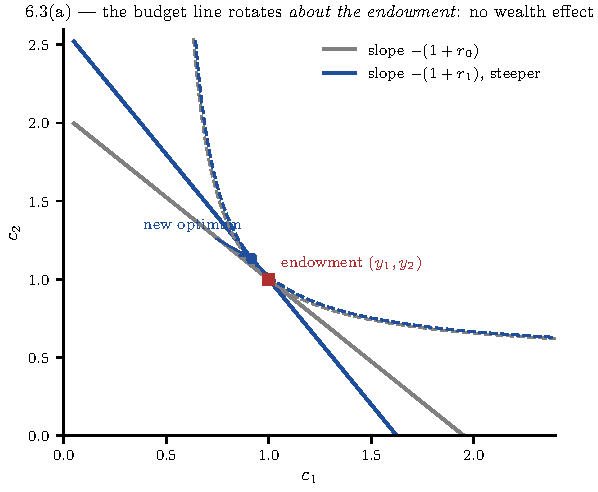
\includegraphics[width=0.72\linewidth]{fig/fig_k6_3_rotacao.pdf}\\[3pt]
\captionof{figure}{Problem 6.3(a). The budget line rotates about the endowment, so the old
bundle stays feasible: pure substitution, $c_1$ falls, utility rises. Drawn with a large
change in $r$ for legibility.}
\label{fig:rot63}
\end{center}
\end{tcolorbox}

%------- 6.6 -------
% Topic: Interest Rates, Income and Substitution Effects
% Keywords: kinked budget set, asymmetric taxation, EIS, income vs substitution, distortion
\begin{tcolorbox}[evenbox,title={Problem 6.6 \quad A Tax on Savings}]
\begin{tcolorbox}[questionbox]
A household solves a special case of the problem from Exercise 6.1, with
$\tau_1=\tau_2=a_0=0$. Suppose now that the government introduces a tax on interest income,
so that a household that saves $a$ (and therefore earns interest $ra$) will have to pay
$\tau ra$ in taxes. (If the household borrows instead of saving it pays no tax.)\\[3pt]
(a) Plot the new budget constraint.\\[3pt]
(b) Show graphically: (i) an example where the new policy persuades households to save more;
(ii) an example where the new policy persuades the household to save less; (iii) an example
where the household does not change its decision in response to the new policy. Explain.
\end{tcolorbox}

\textbf{Solution:}
\begin{enumerate}

\item The tax falls on interest \emph{income} only, so the household faces \textbf{two
different interest rates depending on which side of its endowment it lands on}:
\[
c_2=
\begin{cases}
y_2+\bigl[1+r(1-\tau)\bigr](y_1-c_1), & c_1\le y_1 \quad(\text{saving, }a\ge0),\\[4pt]
y_2+(1+r)(y_1-c_1), & c_1\ge y_1 \quad(\text{borrowing, }a\le0).
\end{cases}
\]
The budget constraint is therefore \textbf{kinked at the endowment point} $(y_1,y_2)$:
\begin{itemize}[leftmargin=1.3em,itemsep=2pt,topsep=3pt]
\item to the \emph{left} of $y_1$ (saving) the slope is $-\bigl[1+r(1-\tau)\bigr]$, which is
      \textbf{flatter} than before --- each unit of saving now buys less future consumption;
\item to the \emph{right} of $y_1$ (borrowing) the slope is unchanged at $-(1+r)$.
\end{itemize}
The endowment point itself is unaffected, since consuming exactly one's income involves no
interest income and hence no tax. The absolute slope increases as $c_1$ increases, so the
budget set remains \textbf{convex} and the first-order conditions can still be used side by
side. See Figure~\ref{fig:imp66}.

\item Because the policy lowers the return to saving, its effect on the \emph{quantity}
saved is exactly the ambiguity of Problem 6.1(e), read in reverse. For a saver, a lower
after-tax return means:
\begin{itemize}[leftmargin=1.3em,itemsep=2pt,topsep=3pt]
\item a \textbf{substitution effect} towards present consumption (future consumption is now
      more expensive): save \emph{less};
\item an \textbf{income effect}: the saver is poorer, so it consumes less of both goods, in
      particular less today: save \emph{more}.
\end{itemize}
Which dominates is governed by $\mathrm{EIS}=1/\sigma$. Hence the three cases.

\begin{enumerate}[label=(\roman*),leftmargin=1.9em,itemsep=5pt,topsep=4pt]
\item \textbf{The household saves more: a saver with a low EIS ($\sigma$ large).} Draw
      sharply curved, almost L-shaped indifference curves. Such a household insists on a
      particular future standard of living; when the return falls it must put aside
      \emph{more} to get there. The income effect dominates.
      \checkmark\ With $y_1=2$, $y_2=0.5$, $\beta=0.97$, $\sigma=5$, $r=0.10$ and
      $\tau=0.5$, saving rises from $a=0.72223$ to $a=0.73398$.

\item \textbf{The household saves less: a saver with a high EIS ($\sigma$ small).} Draw
      nearly straight indifference curves --- the household is close to indifferent about
      \emph{when} it consumes and reacts strongly to the price. The substitution effect
      dominates.
      \checkmark\ Same parameters with $\sigma=0.4$: saving falls from $a=0.81371$ to
      $a=0.76007$.

\item \textbf{The household does not change its decision.} Two clean examples:
      \begin{itemize}[leftmargin=1.2em,itemsep=2pt,topsep=2pt]
      \item \textbf{A borrower.} If the optimum lies to the right of the endowment, it lies
            on the segment the tax never touched, and nothing at all changes. The tax is on
            interest \emph{income}, and this household has none.
            \checkmark\ With $y_1=0.5$, $y_2=2$, $\sigma=2$: $a=-0.69552$ before and after,
            to machine precision.
      \item \textbf{A household exactly at the kink.} At $(y_1,y_2)$ the budget set has a
            corner, so a whole interval of marginal rates of substitution,
            $\bigl[1+r(1-\tau),\,1+r\bigr]$, is consistent with optimality. Any household
            whose MRS at the endowment falls inside that interval stays put --- and the
            interval is \emph{created} by the policy, so the tax actually makes the
            no-trade outcome optimal for a positive measure of households that previously
            saved a little.
      \end{itemize}
\end{enumerate}

\end{enumerate}

\smallskip
\emph{Reading, and the quantity response is the wrong thing to look at.} The exercise is
built to show that the sign of the saving response is not a theoretical result. But three
things about the policy are \emph{not} ambiguous, and they are what a policy discussion
should turn on:

\begin{enumerate}[label=\textbf{\arabic*.},leftmargin=1.6em,itemsep=3pt,topsep=3pt]
\item \textbf{Every saver is strictly worse off.} Its budget set has shrunk, so utility falls
      whatever happens to the quantity saved. Case (i), where the household saves more, is
      not a household that has been made better off --- it is one that has been forced to
      work harder for the same retirement.
\item \textbf{The intertemporal margin is distorted.} At the optimum the saver's MRS equals
      $1+r(1-\tau)$ while the economy's marginal rate of transformation is $1+r$. That wedge
      is a genuine deadweight loss, and it is present in case (i) exactly as much as in case
      (ii). This is a First Welfare Theorem failure of the kind catalogued in \S9.2.
\item \textbf{The asymmetry subsidises debt.} Taxing interest received while leaving interest
      paid untaxed drives a wedge between the borrowing and lending rates, which is a
      distortion on top of the level effect --- and it is exactly the wedge that makes the
      no-trade kink attractive in case (iii).
\end{enumerate}

\begin{center}
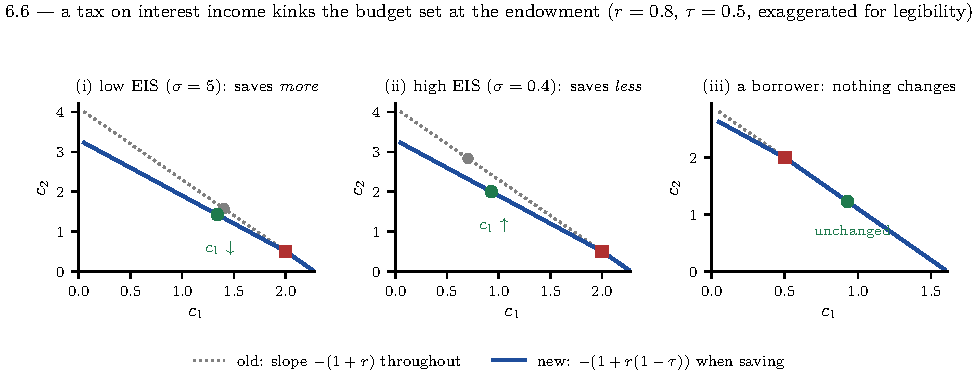
\includegraphics[width=\linewidth]{fig/fig_k6_6_imposto.pdf}\\[3pt]
\captionof{figure}{Problem 6.6. The kinked budget set and the three cases. Green dots are
the new optima. The interest rate is exaggerated so the kink is visible; the signs are the
ones verified numerically at $r=0.10$.}
\label{fig:imp66}
\end{center}
\end{tcolorbox}

%---- Topic: Permanent Income and the Keynesian Consumption Function ----
\subsection{Permanent Income and the Keynesian Consumption Function}

%------- 6.2 -------
% Topic: Permanent Income and the Keynesian Consumption Function
% Keywords: life-cycle income profile, saving rate, borrowers vs savers, human wealth
\begin{tcolorbox}[evenbox,title={Problem 6.2 \quad Savings Rates for Different People}]
\begin{tcolorbox}[questionbox]
An economist has data on the occupation, this year's income (denoted $y$) and this year's
consumption (denoted $c$) of a sample of 26-year-olds. Within this sample, some are top
professional athletes and others are medical doctors in their first year of residence. [Make
whatever assumptions you think are reasonable and, if you wish, refer back to Exercise
6.1.]\\[3pt]
(a) Suppose one computed $s=\dfrac{y-c}{y}$ for each individual in the sample. Should we
expect $s$ to be higher for athletes or doctors?\\[3pt]
(b) Suppose interest rates go down. How should we expect the response of $s$ to differ
between the two groups?
\end{tcolorbox}

\textbf{The assumption that does all the work.} Both groups are 26 years old, so ``this
year's income'' is $y_1$ in the language of Problem 6.1 and everything else is $y_2$. The two
occupations have opposite income profiles:
\begin{center}
\begin{tabular}{@{}lll@{}}
\toprule
 & \textbf{Top athlete, 26} & \textbf{First-year resident, 26} \\
\midrule
Current income $y_1$      & very high (career peak) & very low (a resident's stipend) \\
Future income $y_2$       & low (careers end near 30) & very high (a physician's career) \\
$m=y_2/y_1$               & small                    & large \\
\bottomrule
\end{tabular}
\end{center}
Both are close to the extremes; everything follows from that and from Problem 6.1.

\textbf{Solution:}
\begin{enumerate}

\item From Problem 6.1 with $\tau=a_0=0$,
\[
s=1-\frac{c_1}{y_1}=1-\frac{1}{\Omega}\left(1+\frac{m}{1+r}\right) .
\]
This is \textbf{decreasing in $m$}, so
\[
\boxed{s\ \text{is higher for the athletes.}}
\]
\checkmark\ With $\beta=0.97$, $\sigma=2$, $r=0.06$: an athlete with $(y_1,y_2)=(10,2)$ has
$s=+0.393$; a resident with $(y_1,y_2)=(3,9)$ has $s=-0.958$.

\smallskip
The residents' saving rate is \textbf{negative}, and this is the right prediction rather than
an artefact: first-year residents finance current consumption with student debt. The
athletes save heavily because they know their earning years are nearly over. Neither is a
statement about thrift; both are the same optimising rule applied to opposite income
profiles.

\smallskip
\emph{An important corollary for the economist holding the data.} A cross-sectional
regression of $c$ on $y$ in this sample will find a strong positive relationship and a
declining average propensity to consume, and will be tempted to call it a Keynesian
consumption function. Problem 6.4 shows exactly how that inference fails.

\item Two channels respond to a fall in $r$, and they are of very different sizes for the two
groups.

\begin{enumerate}[label=\textbf{Channel \arabic*.},leftmargin=2.7em,itemsep=4pt,topsep=3pt]
\item \textbf{Human wealth.} $W=y_1+y_2/(1+r)$, so
      $\dd{W}{r}=-y_2/(1+r)^2$: a fall in $r$ raises the present value of future income,
      \emph{in proportion to $y_2$}. This is enormous for the residents, whose income is
      almost all in the future, and negligible for the athletes.
\item \textbf{The price effect.} A fall in $r$ changes $\Omega$, tilting the consumption
      path. Its sign depends on $\sigma$ (Problem 6.1(e)) and its size does not depend on
      the income profile.
\end{enumerate}

Channel 1 dominates the comparison and is unambiguous in sign, so
\[
\boxed{\text{the residents' saving rate falls much more than the athletes'.}}
\]
\checkmark\ Cutting $r$ from $6\%$ to $2\%$: the athlete's $s$ moves by $+0.002$, the
resident's by $-0.038$ --- about \textbf{19 times larger}, and in the opposite direction.

\smallskip
There is also a distributional reading of the same fact. The residents are \emph{borrowers}
($a<0$) and the athletes are \emph{lenders} ($a>0$). A fall in $r$ is a transfer from lenders
to borrowers, so it raises the residents' consumption and lowers the athletes', on top of
the human-wealth channel which points the same way.

\end{enumerate}

\smallskip
\emph{Reading.} This is the microeconomic foundation for one of the most robust findings in
applied macroeconomics: \textbf{the interest sensitivity of consumption is concentrated among
young borrowers with steep income profiles}. It is why monetary policy transmits partly
through household balance sheets rather than uniformly; why the same rate cut has very
different effects in a country with a young, indebted population than in one with an old,
asset-rich one; and why models that assume a single representative household understate the
consumption response to interest rates. Note also that the answer to (b) barely uses
$\sigma$ --- the parameter nobody can estimate --- and rests almost entirely on the income
profile, which is observable.
\end{tcolorbox}

%------- 6.4 -------
% Topic: Permanent Income and the Keynesian Consumption Function
% Keywords: consumption smoothing, cross-section vs time series, APC, Friedman, identification
\begin{tcolorbox}[evenbox,title={Problem 6.4 \quad Consumption and Income}]
\begin{tcolorbox}[questionbox]
Suppose there are two households in the economy. Each of them solves a special case of
Exercise 6.1, where $\tau_1=\tau_2=a_0=0$, $\beta=1$ and $r=0$.\\[3pt]
(a) Solve for $c_1$ as a function of $y_1$ and $y_2$.\\[3pt]
(b) Suppose the incomes of each of the households are:
\begin{center}
\begin{tabular}{@{}lcc@{}}
\toprule
 & $y_1$ & $y_2$ \\
\midrule
Household A & 2 & 4 \\
Household B & 6 & 4 \\
\bottomrule
\end{tabular}
\end{center}
Compute $c_1$ and $c_2$ for each of the households.\\[3pt]
(c) Suppose an economist is trying to decide what is a reasonable model for consumption
behavior and only has data for period 1. Is the data supportive of the Keynesian view of the
consumption function? Explain.\\[3pt]
(d) Suppose the same economist now looks at data for period 2 in addition to data for period
1. Is the data supportive of the Keynesian view of the consumption function? Explain.
\end{tcolorbox}

\textbf{Solution:}
\begin{enumerate}

\item With $\beta=1$ and $r=0$, the Euler equation $c_1^{-\sigma}=\beta(1+r)c_2^{-\sigma}$
collapses to $c_1=c_2$: \textbf{perfect consumption smoothing}, for any $\sigma$.
Equivalently $\Omega=1+1=2$, and the budget constraint is $c_1+c_2=y_1+y_2$, so
\[
\boxed{\;c_1=c_2=\frac{y_1+y_2}{2}\;}
\]
which is average income. Note that neither $\sigma$ nor anything else about preferences
survives: with $\beta(1+r)=1$ the household simply flattens its consumption path.

\item Substituting:
\begin{center}
\begin{tabular}{@{}lrrrrrr@{}}
\toprule
 & $y_1$ & $y_2$ & $c_1$ & $c_2$ & $a=y_1-c_1$ & $\mathrm{APC}_1=c_1/y_1$ \\
\midrule
Household A & 2 & 4 & \textbf{3} & \textbf{3} & $-1$ (borrows) & $1.50$ \\
Household B & 6 & 4 & \textbf{5} & \textbf{5} & $+1$ (saves)   & $0.83$ \\
\bottomrule
\end{tabular}
\end{center}
\checkmark\ Each row satisfies $c_1+c_2=y_1+y_2$ and $c_1=c_2$. Household A has a rising
income profile and borrows against it; household B has a falling one and saves.

\item \textbf{Yes --- and spectacularly so. That is the trap.} With only period-1 data the
economist sees two points, $(y,c)=(2,3)$ and $(6,5)$. Fit a line through them:
\[
\text{slope}=\frac{5-3}{6-2}=0.5,
\qquad
\text{intercept}=3-0.5\times2=2,
\qquad\Longrightarrow\qquad
\boxed{c=2+0.5\,y} .
\]
\checkmark\ This is the Keynesian consumption function $C=\bar C+bY$, and it satisfies every
one of Keynes's stated properties:
\begin{itemize}[leftmargin=1.3em,itemsep=2pt,topsep=3pt]
\item a positive autonomous term, $\bar C=2>0$;
\item a marginal propensity to consume strictly between zero and one, $b=0.5$;
\item an average propensity to consume that \emph{falls} with income, $1.50$ then $0.83$ ---
      the ``fundamental psychological law''.
\end{itemize}
The data were generated by a model in which \textbf{current income does not enter the
consumption decision at all}, and they fit the Keynesian function perfectly. The reason is
that the cross-sectional variation in $y_1$ here is entirely \emph{transitory}: A and B have
the same lifetime income timing but different current income, and the household with
temporarily high income is the one with the low APC. That is precisely Friedman's (1957)
resolution of the cross-section evidence in Figures 6.1.1--6.1.2.

\item \textbf{No. The second period destroys it.} Pool the four observations:
\begin{center}
\begin{tabular}{@{}lcccc@{}}
\toprule
observation & A, period 1 & B, period 1 & A, period 2 & B, period 2 \\
\midrule
income $y$      & 2 & 6 & \textbf{4} & \textbf{4} \\
consumption $c$ & 3 & 5 & \textbf{3} & \textbf{5} \\
\bottomrule
\end{tabular}
\end{center}
The last two columns are fatal: \textbf{the same income, $y=4$, is associated with two
different consumption levels, $3$ and $5$.} No function $c=f(y)$ --- Keynesian, linear, or
otherwise --- can fit that, because a function cannot take two values at one point. The
Keynesian consumption function is not merely mis-estimated; it does not exist for this data.
\checkmark

\smallskip
What \emph{does} fit is immediate once one looks at it the right way: \textbf{within} each
household, income changes ($2\to4$ for A, $6\to4$ for B) and consumption does not move at
all. Consumption is perfectly correlated with lifetime income across households and
perfectly uncorrelated with current income within them.

\end{enumerate}

\begin{tcolorbox}[trapbox]
Do not conclude from (c) that the economist was careless. The period-1 data are real data
correctly summarised; the fitted line has the right slope and the right intercept for the
sample it was estimated on. The error would be \emph{interpreting} the fitted line as a
behavioural relationship --- as something that would still hold if you changed a household's
current income. It would not: hand household A an extra unit of $y_1$ and its consumption
rises by $1/2$ only because the extra unit is permanent-income-relevant; hand it an extra
unit of $y_1$ offset by a unit less of $y_2$ and consumption does not move at all.

\smallskip
This is the identification problem in its cleanest form. The cross-sectional slope of $0.5$
is not the MPC out of any particular kind of income shock; it is an artefact of \emph{what
kind of income variation happens to generate the cross-section}. Change the source of
variation and the slope changes. It is the same reason the aggregate time-series APC is
roughly constant (Kuznets) while the cross-sectional APC falls with income, and reconciling
those two facts is what the permanent income hypothesis was invented to do.
\end{tcolorbox}

\smallskip
\emph{Reading.} Three lessons, in increasing order of generality.
\begin{enumerate}[label=\textbf{\arabic*.},leftmargin=1.6em,itemsep=3pt,topsep=3pt]
\item \textbf{A good fit is not evidence for a mechanism.} The Keynesian function fits data
      generated by a model that contradicts it.
\item \textbf{Panel data beat cross-sections} for consumption questions, because they let you
      hold the household --- and hence its lifetime income --- fixed while current income
      moves. This is why the modern literature is built on panel and administrative data.
\item \textbf{What kind of income shock is it?} Every question about the marginal propensity
      to consume is ill-posed until one says whether the shock is temporary or permanent,
      anticipated or not. Problem 6.8 computes both answers for the infinite-horizon case,
      and the gap between them is an order of magnitude.
\end{enumerate}
\end{tcolorbox}

%---- Topic: Credit Constraints and Ricardian Equivalence ----
\subsection{Credit Constraints and Ricardian Equivalence}

%------- 6.5 -------
% Topic: Credit Constraints and Ricardian Equivalence
% Keywords: borrowing limit, occasionally binding constraint, Ricardian equivalence, fiscal stimulus, MPC
\begin{tcolorbox}[oddbox,title={Problem 6.5 \quad Credit Constraints and Ricardian Equivalence}]
\begin{tcolorbox}[questionbox]
Suppose a household solves the following variant of the problem in Exercise 6.1:
\[
\max_{c_1,\,a,\,c_2}\ u(c_1)+\beta u(c_2)
\quad\text{s.t.}\quad
a=y_1-\tau_1-c_1,
\qquad
c_2=y_2-\tau_2+(1+r)a,
\qquad
a\ge-b
\tag{6.4.1}
\]
(a) What does equation (6.4.1) mean? What does $b$ represent?\\[3pt]
(b) Plot the household's budget constraint. In the same graph, plot constraint
(6.4.1).\\[3pt]
(c) Solve for $c_1$, $c_2$ and $a$.\\[3pt]
(d) Show that, other things being equal, constraint (6.4.1) is more likely to be binding if
(i) $y_2-\tau_2$ is high, (ii) $y_1-\tau_1$ is low, (iii) $b$ is low. Interpret each of these
conditions.\\[3pt]
(e) Suppose that the government announces a stimulus package of size $\Delta$. This involves
lowering $\tau_1$ by $\Delta$ and increasing $\tau_2$ by $\Delta(1+r)$ so that the present
value of taxes is unchanged. How does $c_1$ respond to the stimulus package if we start from
a situation where constraint (6.4.1) is NOT binding? How does $c_1$ respond if we start from
a situation where it IS binding? Explain.\\[3pt]
(f) Suppose that instead of announcing a stimulus package, the government announces that it
will allow households to borrow $\Delta$ from the government and repay it back (with
interest) at $t=2$. How do the effects of this policy compare with the effects of the
stimulus package? Explain.
\end{tcolorbox}

\textbf{Solution:}
\begin{enumerate}

\item \textbf{$a\ge-b$ is a borrowing limit.} Savings $a$ may be negative --- the household
may borrow --- but not below $-b$. So
\[
\boxed{b\ \text{is the maximum amount of debt the household may carry into period 2.}}
\]
$b=0$ means the household cannot borrow at all; $b=\infty$ recovers Problem 6.1. Note what
the constraint is \emph{not}: it is not a solvency condition. The household is perfectly able
to repay --- it will have $y_2-\tau_2$ next period --- and there is no default in the model.
The limit is exogenous, a stand-in for the fact that lenders cannot verify or enforce
repayment out of future labour income. That distinction matters for part (f).

\item In $(c_1,c_2)$ space:
\begin{itemize}[leftmargin=1.3em,itemsep=2pt,topsep=3pt]
\item the \textbf{budget line} is $c_1+\frac{c_2}{1+r}=W$ with
      $W=y_1-\tau_1+\frac{y_2-\tau_2}{1+r}$, a straight line of slope $-(1+r)$ through the
      endowment $(y_1-\tau_1,\,y_2-\tau_2)$;
\item the \textbf{credit constraint} is $a=y_1-\tau_1-c_1\ge-b$, i.e.
      \[
      c_1\le y_1-\tau_1+b ,
      \]
      a \textbf{vertical line}. The feasible set is the part of the budget line to the left
      of it.
\end{itemize}
Note the vertical line always lies weakly to the \emph{right} of the endowment (since
$b\ge0$), so the household can always at least consume its own income. See
Figure~\ref{fig:cred65}.

\item Let $c_1^{u}\equiv W/\Omega$ be the unconstrained solution from Problem 6.1. The
objective is strictly concave in $c_1$ along the budget line, so the constrained maximum is
either interior or at the boundary, and
\[
\boxed{\;c_1=\min\left\{\frac{W}{\Omega},\;y_1-\tau_1+b\right\}\;}
\]
\[
\boxed{\;a=\max\left\{y_1-\tau_1-\frac{W}{\Omega},\;-b\right\}\;},
\qquad
\boxed{\;c_2=y_2-\tau_2+(1+r)a\;}
\]
Explicitly, in the two regimes:
\begin{itemize}[leftmargin=1.3em,itemsep=3pt,topsep=3pt]
\item \textbf{Slack} ($c_1^{u}\le y_1-\tau_1+b$): $c_1=W/\Omega$,
      $c_2=[\beta(1+r)]^{1/\sigma}W/\Omega$, and the Euler equation holds with equality.
\item \textbf{Binding} ($c_1^{u}>y_1-\tau_1+b$): $a=-b$, $c_1=y_1-\tau_1+b$,
      $c_2=y_2-\tau_2-(1+r)b$, and the Euler equation holds as the \emph{inequality}
      $u'(c_1)>\beta(1+r)u'(c_2)$ --- the household would like to move consumption forward
      and cannot.
\end{itemize}
That last inequality is the signature of a constrained household and is what the empirical
literature looks for.

\item The constraint binds iff $W/\Omega>y_1-\tau_1+b$. Multiply out and collect:
\[
\frac{y_1-\tau_1+\frac{y_2-\tau_2}{1+r}}{\Omega}>y_1-\tau_1+b
\]
\[
\Longleftrightarrow\qquad
\boxed{\;\frac{y_2-\tau_2}{1+r}\;>\;(\Omega-1)(y_1-\tau_1)+\Omega\,b\;}
\tag{6.5.1}
\]
with $\Omega-1=\beta^{1/\sigma}(1+r)^{(1-\sigma)/\sigma}>0$ and $\Omega>1$. \checkmark\
Condition (6.5.1) is checked against direct solution of the constrained problem for five
different parameter configurations in \texttt{ch06\_numerico.py}.

\smallskip
Every coefficient in (6.5.1) is positive, so the three claims can be read straight off it:
\begin{enumerate}[label=\textbf{(\roman*)},leftmargin=2.1em,itemsep=4pt,topsep=3pt]
\item \textbf{$y_2-\tau_2$ high $\Rightarrow$ binds.} The left-hand side rises. A household
      that expects to be much richer later \emph{wants} to borrow against that; the more it
      wants, the more likely the limit stops it. This is the medical resident of Problem 6.2,
      and it is why credit constraints bite hardest on exactly the households whose lifetime
      income is highest relative to their current income --- students, young professionals,
      anyone at the start of a steep career.
\item \textbf{$y_1-\tau_1$ low $\Rightarrow$ binds.} The right-hand side falls. With little
      current income, almost all of desired consumption has to be financed by borrowing.
      Note that $\tau_1$ enters symmetrically with $-y_1$: \emph{a tax today can itself push
      a household into the constrained region}, which is the whole point of part (e).
\item \textbf{$b$ low $\Rightarrow$ binds.} Mechanical, and it is the policy variable. $b$
      is a measure of financial development: how much can a household borrow against future
      income? Cross-country and cross-time variation in $b$ --- credit-card penetration,
      student-loan availability, mortgage loan-to-value limits --- is the standard
      explanation for why the same income shock produces very different consumption
      responses in different places and decades.
\end{enumerate}

\item \textbf{A present-value-neutral tax cut.} The package sets $\tau_1\to\tau_1-\Delta$ and
$\tau_2\to\tau_2+\Delta(1+r)$, so the present value of taxes changes by
\[
-\Delta+\frac{\Delta(1+r)}{1+r}=0
\qquad\Longrightarrow\qquad
W\ \text{is unchanged.}
\]

\begin{enumerate}[label=\textbf{(\roman*)},leftmargin=2.1em,itemsep=5pt,topsep=4pt]
\item \textbf{Constraint slack: $c_1$ does not move at all.} $c_1=W/\Omega$ and $W$ is
      unchanged, so
      \[
      \boxed{\dd{c_1}{\Delta}=0} .
      \]
      The household saves the entire tax cut --- $a$ rises by exactly $\Delta$ --- in order
      to pay the higher tax next period. This is \textbf{Ricardian equivalence}: the timing
      of lump-sum taxes is irrelevant, because the household undoes it. \checkmark

\item \textbf{Constraint binding: $c_1$ rises one-for-one.} Now
      $c_1=y_1-\tau_1+b$, and $\tau_1$ has fallen by $\Delta$:
      \[
      \boxed{\dd{c_1}{\Delta}=1} .
      \]
      The marginal propensity to consume out of the stimulus is \textbf{one}. \checkmark\
      Numerically, with $\beta=0.96$, $\sigma=2$, $r=0.05$, $\Delta=0.2$: an unconstrained
      household's $c_1$ stays at $2.02046$; a constrained one's rises from $1.05$ to $1.25$,
      exactly $\Delta$.
\end{enumerate}

\smallskip
\emph{The explanation, and it is the point of the whole problem.} Ricardian equivalence is
not a claim about people being clever or far-sighted. It is a claim that the tax cut has
given the household nothing it did not already have: the ability to move a unit of resources
from period 2 to period 1 at the rate $1+r$. An unconstrained household could already do
that in the credit market, so the government's offer is redundant and is neutralised. A
constrained household could \emph{not} do it, and for that household the tax cut is not a
transfer of timing --- it is a \textbf{relaxation of a binding quantity constraint}, which
is why the whole thing is spent.

\item \textbf{A government loan of $\Delta$ is exactly the same policy.} Allowing the
household to borrow $\Delta$ from the government and repay $(1+r)\Delta$ at $t=2$ raises the
borrowing limit from $b$ to $b+\Delta$, so
\[
c_1=\min\left\{\frac{W}{\Omega},\;y_1-\tau_1+b+\Delta\right\} .
\]
Therefore:
\begin{itemize}[leftmargin=1.3em,itemsep=3pt,topsep=3pt]
\item if the constraint was slack, \textbf{nothing happens}: an extra credit line that the
      household did not want is worthless;
\item if it was binding, $c_1$ rises by exactly $\Delta$ --- \textbf{identical to the
      stimulus package}.
\end{itemize}
\checkmark\ Verified numerically: for both household types, $c_1$ under the loan equals
$c_1$ under the tax cut, to machine precision.

\smallskip
\emph{The comparison, and it reframes what fiscal stimulus is.} The two policies have the
same effect because \textbf{they are the same policy}. Cutting $\tau_1$ by $\Delta$ and
raising $\tau_2$ by $\Delta(1+r)$ \emph{is} lending $\Delta$ at rate $r$ and collecting it
back. The label ``stimulus'' is doing no work; the mechanism is credit provision, and it
operates only through households whose credit constraint binds.

\smallskip
Two consequences worth drawing out:
\begin{itemize}[leftmargin=1.3em,itemsep=3pt,topsep=3pt]
\item \textbf{The government's comparative advantage is enforcement, not spending.} Private
      lenders will not lend more than $b$ because they cannot compel repayment out of future
      income. The government can --- through the tax system. That, and not any demand-side
      story, is what makes the policy work in this model.
\item \textbf{The loan is better targeted.} The tax cut moves everyone's taxes, including the
      unconstrained households who simply save it; the loan is voluntary, so only the
      households that would respond take it up. In this model the two give the same $c_1$,
      but the loan achieves it without moving the tax bill of anyone who does not need it.
\end{itemize}

\smallskip
The general moral is the one \S9.2 states as a rule: identify which assumption of the First
Welfare Theorem fails before recommending a policy. Here the failure is \emph{incomplete
markets / borrowing constraints}, and once that is named, the effective policy --- relax the
constraint --- follows immediately, while policies aimed at anything else do nothing.

\end{enumerate}

\begin{center}
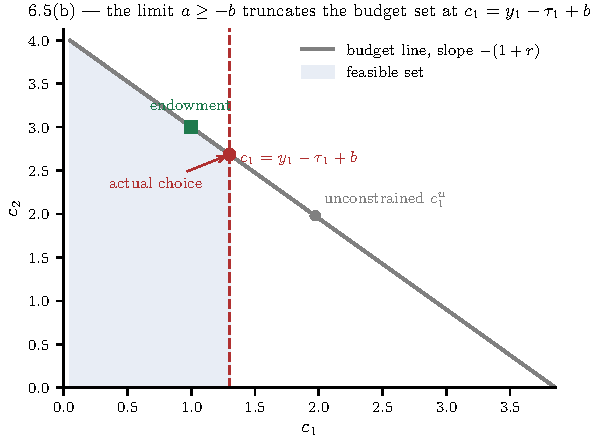
\includegraphics[width=0.72\linewidth]{fig/fig_k6_5_credito.pdf}\\[3pt]
\captionof{figure}{Problem 6.5(b). The borrowing limit truncates the budget set with a
vertical line at $c_1=y_1-\tau_1+b$. Here the household would like $c_1^{u}$ and is pushed
back to the boundary.}
\label{fig:cred65}
\end{center}
\end{tcolorbox}

%---- Topic: Many Periods, and Optimal Saving in a Solow Economy ----
\subsection{Many Periods, and Optimal Saving in a Solow Economy}

%------- 6.8 -------
% Topic: Many Periods, and Optimal Saving in a Solow Economy
% Keywords: infinite horizon, annuity, permanent income hypothesis, MPC, geometric sums
\begin{tcolorbox}[evenbox,title={Problem 6.8 \quad The Marginal Propensity to Consume}]
\begin{tcolorbox}[questionbox]
Suppose a household has preferences given by (6.3.1) over consumption across infinite
periods. Its discount factor and the real interest rate satisfy
\[
1+r=\frac{1}{\beta} .
\]
The household starts with no wealth, will receive income $y_0$ in period $t=0$ and income
$\bar y$ in every subsequent period, from $t=1$ onwards.\\[3pt]
(a) Use the Euler equation (6.3.9) and the budget constraint (6.3.8) to find an expression
for initial-period consumption $c_0$.\\[3pt]
(b) Compute $c_0/y_0$.\\[3pt]
(c) Suppose $r=0.04$. What is the marginal propensity to consume out of a purely temporary
increase in income? Describe in words what a household does with a temporary increase in
income.
\end{tcolorbox}

\textbf{Solution:}
\begin{enumerate}

\item \textbf{Step 1: the Euler equation flattens the path.} Equation (6.3.9) is
$u'(c_t)=\beta(1+r)u'(c_{t+1})$. With $\beta(1+r)=1$ this is $u'(c_t)=u'(c_{t+1})$, and
since $u'$ is strictly decreasing,
\[
c_t=c\quad\text{for every }t .
\]
Consumption is \emph{perfectly flat}, whatever $\sigma$ is and whatever the income path
looks like. Note how much this assumption buys: it removes preferences from the problem
entirely and leaves pure accounting.

\smallskip
\textbf{Step 2: write the budget constraint.} Equation (6.3.8) with $a_0=0$ is
\[
\sum_{t=0}^{\infty}\frac{c_t}{(1+r)^t}=\sum_{t=0}^{\infty}\frac{y_t}{(1+r)^t} .
\]
The left-hand side is a geometric sum with ratio $1/(1+r)<1$:
\[
\sum_{t=0}^{\infty}\frac{c}{(1+r)^t}=\frac{c}{1-\frac{1}{1+r}}=c\,\frac{1+r}{r} .
\]
The right-hand side splits into the first term and the rest:
\[
y_0+\sum_{t=1}^{\infty}\frac{\bar y}{(1+r)^t}
=y_0+\frac{\bar y}{1+r}\cdot\frac{1}{1-\frac{1}{1+r}}
=y_0+\frac{\bar y}{r} .
\]

\smallskip
\textbf{Step 3: solve.}
\[
c\,\frac{1+r}{r}=y_0+\frac{\bar y}{r}
\qquad\Longrightarrow\qquad
\boxed{\;c_0=c=\frac{r}{1+r}\left(y_0+\frac{\bar y}{r}\right)=\frac{r\,y_0+\bar y}{1+r}\;}
\]
\checkmark\ Verified in \texttt{ch06\_numerico.py} by simulating $4000$ periods of the asset
recursion $a_{t+1}=(1+r)a_t+y_t-c_0$ and confirming that the present value of consumption
equals the present value of income to $10^{-6}$.

\smallskip
\emph{Two readings of the same formula, and the second is the useful one.} Write the answer
as
\[
c_0=\underbrace{\bar y}_{\text{permanent income}}
+\underbrace{r\cdot\frac{y_0-\bar y}{1+r}}_{\text{interest on the annuitised windfall}} .
\]
The household treats the excess $y_0-\bar y$ as a windfall, saves it, and consumes only the
interest on it, forever. \checkmark\ Indeed the simulated asset path settles at exactly
$a=(y_0-\bar y)/(1+r)$ and stays there.

\item Dividing by $y_0$,
\[
\boxed{\;\frac{c_0}{y_0}=\frac{r\,y_0+\bar y}{(1+r)\,y_0}
=\frac{r}{1+r}+\frac{1}{1+r}\cdot\frac{\bar y}{y_0}\;}
\]
This is a consumption function --- but of the \emph{ratio} $\bar y/y_0$, not of the level of
$y_0$. A household with an unusually good year ($y_0>\bar y$) has a low APC and a household
with an unusually bad one has an APC above one, which is exactly the cross-sectional pattern
Problem 6.4 produces and Keynes misread.

\item \textbf{The marginal propensity to consume out of temporary income.} A ``purely
temporary'' increase raises $y_0$ and leaves $\bar y$ alone:
\[
\pd{c_0}{y_0}=\frac{r}{1+r}=\frac{0.04}{1.04}=\boxed{0.0385}
\qquad\text{i.e.\ }3.85\% .
\]
\checkmark

\smallskip
\textbf{In words:} the household receives an extra dollar, \textbf{saves 96.2 cents of it},
and consumes 3.8 cents. It then goes on consuming an extra 3.8 cents \emph{every year
forever}, financed by the interest on the 96.2 cents it put away. It converts the windfall
into an annuity and lives off the coupon --- because a one-off dollar, spread over an
infinite life, is worth only its annuity value.

\smallskip
\emph{Contrast with a permanent increase}, where $y_0$ and $\bar y$ both rise by one:
\[
\pd{c_0}{y_0}+\pd{c_0}{\bar y}=\frac{r}{1+r}+\frac{1}{1+r}=\boxed{1} .
\]
\checkmark\ The permanent MPC is exactly one; the temporary MPC is $r/(1+r)$. At $r=4\%$
these differ by a \textbf{factor of 26}.

\end{enumerate}

\smallskip
\emph{Reading --- this is both the model's cleanest prediction and its biggest problem.}

\begin{enumerate}[label=\textbf{\arabic*.},leftmargin=1.6em,itemsep=4pt,topsep=3pt]
\item \textbf{The prediction is unusually sharp.} It contains no preference parameters at
all: $\sigma$ cancelled at the Euler equation, $\beta$ was pinned by $\beta(1+r)=1$. The
number $r/(1+r)$ is pure arithmetic, which makes it a genuine test of the theory rather than
a calibration.

\item \textbf{The test fails, and not narrowly.} Measured responses to temporary transfers
--- tax rebates, stimulus cheques, lottery wins, anticipated tax refunds --- come in around
$0.2$ to $0.6$ in the quarter of receipt, five to fifteen times the $0.038$ predicted here.
The gap is far too large to be measurement error.

\item \textbf{The two repairs are the rest of the chapter.} Either the household \emph{cannot}
save the windfall's counterpart --- it is up against a borrowing constraint and has been
consuming less than it wants (Problem 6.5, where the MPC out of exactly this kind of transfer
is \textbf{one}) --- or it does not do the calculation at all (\S6.4, behavioural theories:
rational inattention, mental accounting, self-control). The modern literature mostly takes
the first route, and Problem 6.5(e) is the reason: constraints deliver the observed MPCs
without abandoning optimisation.

\item \textbf{The infinite horizon is doing real work.} With a finite horizon $T$ the same
derivation gives an MPC of roughly $1/T$ rather than $r/(1+r)$ --- larger, and larger still
for households near the end of life. Part of the measured MPC is therefore just the fact
that people do not live forever.
\end{enumerate}
\end{tcolorbox}

%------- 6.7 -------
% Topic: Many Periods, and Optimal Saving in a Solow Economy
% Keywords: Golden Rule, dynamic inefficiency, negative interest rate, Euler equation, partial equilibrium
\begin{tcolorbox}[oddbox,title={Problem 6.7 \quad One Rational Household}]
\begin{tcolorbox}[questionbox]
Consider an economy that is well described by the Solow growth model. The production
function is $Y=K^{\alpha}L^{1-\alpha}$. The population is constant and equal to 1 and there
is no technological progress. The saving rate is $s$ and the depreciation rate is
$\delta$.\\[3pt]
(a) What will the capital stock be in the long run?\\[3pt]
(b) What will be the real interest rate in the long run?\\[3pt]
For the rest of the question, assume that $s=0.4$, $\alpha=0.35$ and $\delta=0.1$ and the
economy is initially at a steady state.\\[3pt]
(c) If the savings rate increases from $s=0.4$ to $s=0.5$: (i) Will GDP increase in the long
run? (ii) Will consumption increase in the long run?\\[3pt]
(d) Suppose a single household in the economy (the Friedmans) decides that, instead of just
saving an exogenous fraction $s$ of their income, they are going to start choosing
consumption and saving to maximize $\sum_{t=0}^{\infty}\beta^{t}u(c_t)$. The Friedmans can
borrow or lend at the market interest rate. Since it's just the Friedmans who start acting
this way, and they are small relative to the economy, we are going to assume that the
aggregate economy (aggregate quantities, prices, etc.) remains unchanged. Will the
Friedmans' consumption be high initially and then fall over time, be low initially and then
rise over time, or remain constant?
\end{tcolorbox}

\textbf{Solution:}
\begin{enumerate}

\item With $L=1$, $n=g=0$, the steady state has $sY=\delta K$:
\[
sK^{\alpha}=\delta K
\qquad\Longrightarrow\qquad
\boxed{K\stst=\left(\frac{s}{\delta}\right)^{\frac{1}{1-\alpha}}},
\qquad
Y\stst=\left(\frac{s}{\delta}\right)^{\frac{\alpha}{1-\alpha}} .
\]

\item $r=F_K-\delta=\alpha K^{\alpha-1}-\delta$. Evaluating at $K\stst$, and using
$(K\stst)^{\alpha-1}=\delta/s$ from the steady-state condition,
\[
\boxed{\;r=\alpha\,\frac{\delta}{s}-\delta=\delta\,\frac{\alpha-s}{s}\;}
\]
\checkmark\ Note immediately what this says: \textbf{the sign of $r$ is the sign of
$\alpha-s$}. The interest rate is negative precisely when the saving rate exceeds the capital
share --- which is the Golden Rule condition of Problem 5.8, met again from the price side.

\item With $\alpha=0.35$, $\delta=0.1$:
\begin{center}
\begin{tabular}{@{}rrrrr@{}}
\toprule
$s$ & $K\stst$ & $Y\stst$ & $c\stst=(1-s)Y\stst$ & $r$ \\
\midrule
$0.35=\alpha$ & 6.8711 & 1.9632 & \textbf{1.2761} & $\hphantom{+}0.0000$ \\
0.40 & 8.4381 & 2.1095 & 1.2657 & $-0.0125$ \\
0.50 & 11.8943 & 2.3789 & 1.1894 & $-0.0300$ \\
\bottomrule
\end{tabular}
\end{center}
\checkmark

\begin{enumerate}[label=(\roman*),leftmargin=1.9em,itemsep=4pt,topsep=3pt]
\item \textbf{GDP rises: yes.} $Y\stst$ is increasing in $s$ always, from $2.1095$ to
      $2.3789$, a gain of $12.8\%$. More saving always buys more capital and more output.

\item \textbf{Consumption falls: no.} $c\stst=(1-s)(s/\delta)^{\alpha/(1-\alpha)}$ is
      maximised at the Golden Rule $s_{gr}=\alpha=0.35$, and the economy is \emph{already
      past it}. Raising $s$ from $0.4$ to $0.5$ lowers $c\stst$ from $1.2657$ to $1.1894$, a
      loss of $6.0\%$.
      \checkmark\ A grid search over $s\in(0,1)$ locates the maximum at $s=\alpha$ to four
      digits.
\end{enumerate}

\smallskip
This economy is \textbf{dynamically inefficient}: it could raise consumption in \emph{every}
period, starting immediately, simply by saving less. There is no trade-off to weigh --- it is
over-accumulating, and the negative interest rate in part (b) is the price signal saying so.
Note the contrast with Problem 5.8, where $s=0.2<\alpha=0.6$ and the economy was on the other
side.

\item \textbf{High initially, then falling forever.}

\smallskip
The Friedmans take $r$ as given at the steady-state value from part (b),
\[
r=\delta\,\frac{\alpha-s}{s}=0.1\times\frac{0.35-0.40}{0.40}=-0.0125 ,
\]
and their Euler equation (6.3.9) with CRRA utility gives the growth factor of their
consumption:
\[
\frac{c_{t+1}}{c_t}=\bigl[\beta(1+r)\bigr]^{\frac{1}{\sigma}} .
\]
Now $1+r=0.9875<1$ and $\beta<1$, so
\[
\beta(1+r)<1
\qquad\Longrightarrow\qquad
\boxed{\;\frac{c_{t+1}}{c_t}<1\ \text{ for every }\beta<1\text{ and every }\sigma>0\;}
\]
\checkmark\ Checked for $\beta\in\{0.90,0.96,0.99,0.999\}$ and
$\sigma\in\{0.5,1,2,5\}$; every combination gives a factor below one. With $\beta=0.96$ and
$\sigma=2$ the factor is $0.97365$, so the Friedmans' consumption falls by about
$2.6\%$ a year.

\smallskip
\emph{Why the answer is unambiguous, which it usually is not.} Ordinarily the sign of
consumption growth is a race between impatience ($\beta<1$, pushing consumption forward) and
the return on saving ($1+r$, pushing it back). Here the return is \emph{itself} below one:
saving physically destroys resources, because the marginal product of capital is less than
depreciation. Both forces point the same way, so no assumption about $\beta$ or $\sigma$ is
needed. The Friedmans consume more than their Solow neighbours today, run their wealth down,
and converge geometrically towards zero consumption relative to them.

\end{enumerate}

\smallskip
\emph{Reading --- what this exercise is really demonstrating.}

\begin{enumerate}[label=\textbf{\arabic*.},leftmargin=1.6em,itemsep=4pt,topsep=3pt]
\item \textbf{The exogenous saving rate is a genuinely restrictive assumption, and the model
tells you so.} No optimising household would choose $s=0.4$ here. Given the prices this
economy generates, the rational response is to save \emph{less} than everybody else --- the
Solow assumption is not just arbitrary, it is inconsistent with the behaviour of anyone who
looks at the interest rate.

\item \textbf{Part (d) is a partial-equilibrium thought experiment, and it must be.} If all
households became Friedmans, aggregate saving would fall, $K$ would fall, $F_K$ would rise
and $r$ would rise, until $\beta(1+r)=1$ and consumption stopped falling. That is exactly the
steady state of Chapter 9:
\[
F_K(K\stst,1)-\delta=\frac{1}{\beta}-1>0 ,
\]
which is \emph{strictly below the Golden Rule} and therefore has a strictly positive interest
rate. The general-equilibrium version can never be dynamically inefficient; only an
exogenous saving rate can produce that. Problem 9.11 works this out.

\item \textbf{The declining path is not a paradox.} It looks strange that a household
optimising over an infinite horizon plans for its own consumption to fall forever, but it is
the correct response to a negative return: there is no way to store value, so the best plan
front-loads. The Friedmans are not making a mistake; the economy they live in is.
\end{enumerate}

\begin{center}
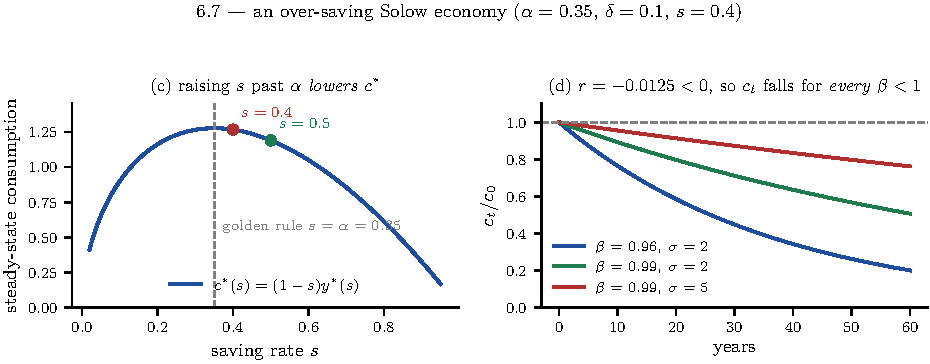
\includegraphics[width=\linewidth]{fig/fig_k6_7_solow.pdf}\\[3pt]
\captionof{figure}{Problem 6.7. Left: steady-state consumption peaks at $s=\alpha=0.35$, so
moving from $0.4$ to $0.5$ goes downhill. Right: with $r<0$ the Friedmans' consumption
declines for every discount factor.}
\label{fig:solow67}
\end{center}
\end{tcolorbox}

%======================================================================
\section*{Companion code}
\addcontentsline{toc}{section}{Companion code}
%======================================================================

Every numerical result above is reproduced by \texttt{Resolucao/kurlat\_ch06\_codigo/}. Each
script checks its analytical formulas against an independent numerical computation and aborts
on any mismatch.

\begin{center}
\begin{tabular}{@{}lp{10.2cm}@{}}
\toprule
\textbf{File} & \textbf{What it does} \\
\midrule
\texttt{ch06\_numerico.py} & Problem 6.1: the closed form checked against a direct numerical
maximisation of $u(c_1)+\beta u(c_2)$ over the budget line, for four values of $\sigma$, plus
finite-difference confirmation of all four comparative statics and of the sign rule
$\operatorname{sign}\dd{c_1}{r}=\operatorname{sign}(\sigma-1)$. Problem 6.9: homotheticity
and the elasticity $y_1/W$, over a grid in $m$ and $r$. Problem 6.3: $\beta$ calibrated so
the household sits exactly at its endowment, then $c_1\downarrow$, $a>0$ and $U\uparrow$
verified. Problem 6.6: the kinked budget set solved by comparing both segments, producing the
three cases. Problem 6.2: the two income profiles, their saving rates and their responses to
a rate cut. Problem 6.4: perfect smoothing, the Keynesian fit $c=2+0.5y$, and the pooled data
that admit no consumption function. Problem 6.5: the closed-form binding condition (6.5.1)
checked against direct solution, the three monotonicity claims, and the equivalence of the
tax cut and the government loan. Problem 6.8: a 4000-period simulation confirming the flat
path, the annuitised windfall and both MPCs. Problem 6.7: the steady state, the golden-rule
grid search, and the Euler growth factor for a grid of $\beta$ and $\sigma$. \\
\texttt{ch06\_figuras.py} & The five figures. \\
\texttt{estilo\_mpl.py} & \texttt{pgf} backend, so figure text is typeset by \texttt{pdflatex}
with \texttt{lmodern} and \texttt{cmap} and the PDF stays fully copyable. \\
\bottomrule
\end{tabular}
\end{center}

\end{document}
